%%%%%%%%%%%%%%%%%%%%%%%%%%%%%%%%%%%%%%%%%%%%%%%%%%%%%%%%%%%%%%%%%%%%%%%%%%%%%%%%
%% Title (en): Multiagent Systems and Organizations                           %%
%% Title (cs): Multiagentní systémy a organizace                              %%
%%                                                                            %%
%% Author: Bc. Lukáš Kúdela                                                   %%
%% Supervisor: Prof. RNDr. Petr Štěpánek, DrSc.                               %%
%%                                                                            %%
%% Academic year: 2011/2012                                                   %%
%%%%%%%%%%%%%%%%%%%%%%%%%%%%%%%%%%%%%%%%%%%%%%%%%%%%%%%%%%%%%%%%%%%%%%%%%%%%%%%%

% TODO Rename to Organization-Centric MAS Metamodels
\chapter{Poor Model Problem and its Solutions}

%%%%%%%%%%%%%%%%%%%%%%%%%%%%%%%%%%%%%%%%%%%%%%%%%%%%%%%%%%%%%%%%%%%%%%%%%%%%%%%%
%% Agent UML                                                                  %%
%%%%%%%%%%%%%%%%%%%%%%%%%%%%%%%%%%%%%%%%%%%%%%%%%%%%%%%%%%%%%%%%%%%%%%%%%%%%%%%%
\section{Agent UML}

% OOSE and UML
In the field of object-oriented software engineering (OOSE), to describe the design of an object-oriented system (OOS) in a universally understood way, Unified Modelling Language (UML) is used.
UML is a standardized general-purpose modelling language for OOSE.
It standard was created (and is managed) by the Object Management Group (OMG).
It has several essential properties and capabilities that contribute to its popularity.

First and foremost, UML is programming language agnostic.
This may seem unnecessary since usually by the time the system is designed the programming language will already have been chosen and thus the freedom to change it later (in the implementation phase) is not required.
However, even if the programming (or implementation) language is well beforehand (and is not likely to change), it can still be convenient to abstract from it in the design phase to be able to ignore the implementation details of that particular programming language.

Secondly, UML can be used to model both structural (static) and behavioural (dynamic) aspects of an OOS.
Examples of structural aspects are the class and object structures, while an example of a dynamic aspect is the object interaction.

Thirdly, the designer can choose how much they commit to using UML.
Even though UML is semantically rich enough to support advanced software engineering practices like formal verification (software verification), code generation and metamodelling, the designer can choose to employ its graphic notation techniques to sketch visual models of an OOS.

% AOSE and AUML

The field of agent-oriented software engineering (AOSE) deals with agent-oriented systems (AOS).
The AOS's (multiagent systems) can be characterized as extensions of OOS's; after all, an agent is basically a special kind of object - an autonomous object.
This means that we should be able to use UML to describe MAS.

However, it turns out that MAS represent a too big a paradigm shift from classical object-oriented programming (OOP) for UML itself to handle.
The problem is that AOSE adds another layer of abstractions (abstraction layer) over the traditional OOSE.
Attempting to talk or write about these (higher-level) abstractions in terms of (lower-level) UML would obfuscate their true nature.
The situation calls for a higher-level modelling language based on UML.

Agent UML (AUML) [AUML: http://www.auml.org/], an extension of UML, has been developed by FIPA Modeling Technical Comitte [FIPA-MTC: http://www.fipa.org/activities/modeling.html] to facilitate the modelling of AOS's in AOSE.
According to its authors, AUML does not want to be restricted by UML; it only wants to capitalize on it where it can.
This in practice means, that instead of strict reliance on the UML as defined by OMG, the AUML's designers intend to reuse portions of UML where it makes sense.

% AUML effort halted
The current situation of AUML can be described as quiescent [] mostly because other initiatives (UML 2.1, OMG Systems Modeling Language,  OMG UML Metamodel and Profile for Services RFP) have already delivered or are poised to deliver features AUML itself intended to provide.

Altough there is not much effort going into AUML at the moment, we have decided to use it as the modelling language in this thesis.
The decision is motivated by the fact that we will only use the modelling language to create visual models and AUML is the simplest language enabling that.
The remainder of this section is devoted to introducing parts of AUML relevant to us.

%%%%%%%%%%%%%%%%%%%%%%%%%%%%%%%%%%%%%%%%%%%%%%%%%%%%%%%%%%%%%%%%%%%%%%%%%%%%%%%%
%% Aalaadin/AGR                                                               %%
%%%%%%%%%%%%%%%%%%%%%%%%%%%%%%%%%%%%%%%%%%%%%%%%%%%%%%%%%%%%%%%%%%%%%%%%%%%%%%%%
\section{Aalaadin/AGR}

% Aallaadin/AGR - references
This section introduces the Aalaadin/AGR\footnote{`Aalaadin' is the old name, whereas `AGR' is the new one. Since it is arguably fancier, we will use the old name.} metamodel described in \cite{Ferber97}, \cite{Ferber98}, \cite{Ferber00} and \cite{Ferber03}.
The overview presented here is particularly after \cite{Ferber98}.

% Aalaadin/AGR - authors
Aalaadin/AGR has been proposed in 1997 by Jacques Ferber, Oliver Gutknecht and their colleagues from Montpellier 2 University in Montpellier, France.

%% Summary %%%%%%%%%%%%%%%%%%%%%%%%%%%%%%%%%%%%%%%%%%%%%%%%%%%%%%%%%%%%%%%%%%%%%

- PIM

% Aalaadin - about
Aalaadin is a platform-independent (ALT: generic) metamodel of multiagent systems based on three core concepts: agent, group and role.
It is actually what its authors refer to as \textit{organization-centric multiagent system} (OCMAS) metamodel, because it enables a MAS designer to build/describe/specify various organization models such as flat (e.g. market-like) or hierarchical (e.g. enterprise-like) organizations.

In the following subsections, the Aalaadin metamodel (called simply model) will be introduced.
The model itself has two levels:
\begin{itemize}
	\item The \textbf{concrete level} contains relatively concrete concepts like \textit{agent}, \textit{group} and \textit{role}.
	The language defined by this level is used to describe concrete organizations.
	\item The \textbf{abstract level} contains more abstract concepts like \textit{group structure}, \textit{organization structure} and \textit{interaction}. 
	The language of this level is used to describe abstract organizations, i.e. families of organizations sharing the same structural characteristics.
\end{itemize}

% TODO Concrete organization vs. abstract organization
To understand the following text, it is essential to make a distinction between a \textit{concrete organization} and \textit{abstract organization}.
A concrete organization is the actual organization that exists in a MAS at run-time, whereas an abstract organization is the organization specification that exists in a MAS at design-time.
To put it differently, an abstract organization represents a (possibly infinite) set of all imaginable organizations conforming to common specification and a concrete organization represents a member of this set.

% Organization instance vs organization class
Later we will use the terms \textit{organization instance} and \textit{organization class} to refer to an concrete organization and abstract organization respectively.
These terms try to capture the essence of the relationship between an abstract and concrete organization (namely, a concrete organization being an instance of an abstract organization and conversely, an abstract organization being a class of a concrete organization) and are imported from OOP where it is necessary to make a similar distinction. 

%%%%%%%%%%%%%%%%%%%%%%%%%%%%%%%%%%%%%%%%%%%%%%%%%%%%%%%%%%%%%%%%%%%%%%%%%%%%%%%%
\subsection{Core Concepts}

% Core model - about
The Aalaadin core model is based on three \textit{core concepts}: \textit{agent}, \textit{group} and \textit{role}.
Figure~\ref{figure:aalaadin-core-model} shows a diagram of the core model.

% Figure: Aalaadin core model
\begin{figure}[h]
	\centering
	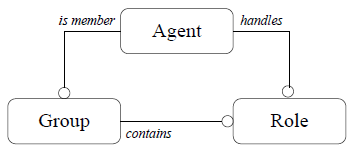
\includegraphics[width=0.5\textwidth]{images/aalaadin-core-model.png}
	\caption{The Aalaadin core model}
	\label{figure:aalaadin-core-model}
\end{figure}

\subsubsection*{Agent}

% Agent - definition
An \textit{agent} is defined in \cite{Ferber97} as an active communicating entity which plays \textit{roles} within \textit{groups}.

% Agent - no agent architecture imposed
The Aalaadin model does not prescribe any particular agent architecture.
Any metamodel striving for generality should impose as little constraints upon the MAS designer as possible.
After all, the decision of which agent architecture to use is best made by the designers themselves and relates to the MAS as such, not just its organizational structure.
As we will see, none of the metamodels introduced in this thesis force the MAS designers to adapt a concrete definition of agenthood.

\subsubsection*{Group}

% Group - definition
In \cite{Ferber97}, \textit{groups} are defined as atomic sets of agent aggregation.
Each agent belongs to one (possibly none) or more groups.

% Group - about
In its most basic form, a group is just a way to tag a set of agents, i.e. it has no structure.
The real advantage of grouping agents becomes apparent when we introduce some order \footnote{The casual, not formal, meaning of the word is intended here.} to these groups.
This order can be achieved using roles.

% Group - characteristics
Groups have the following characteristics:
\begin{itemize}
	\item An agent can be a member of any number of groups simultaneously.
	This means that group can overlap, which is major point of Aalaadin.
	\item A new group can be founded by any agent and an agent must request its admission to an existing group.
	\item A group may be local or distributed across multiple machines.
\end{itemize}

\subsubsection*{Role}

% Role - definition
A \textit{role} is an abstract representation of n agent function, service or identification within a group \cite{Ferber97}.
An agent can play multiple roles each of which is local to a group.
Similarly to group admission, playing a group in a role must be requested by the candidate agent (already belonging to the group) and awarded by the founder agent.

% Role & communication
In Aalaadin, the communication is related to roles. Since an agent can play multiple roles, the model allows it to engage in multiple independent dialogs simultaneously.

% Role - definition characteristics
The following characteristics are part of a role definition:
\begin{itemize}
	\item \textit{uniqueness}. A role can be \textit{unique} or \textit{multiple} within a group.
	A unique role can be played by at most one agent in a given group.
	A multiple role, on the other hand, can be played by any number of agents in a given group. 
	\item a list of competences. A \textit{competence} specifies a condition the candidate agent must satisfy to be eligible to play the role within the group. 
	\item a list of capacities. A \textit{capacity} specifies an ability attributed to an agent while it is playing the role.
\end{itemize}
By default a role is multiple, does not require any competences and does not provide any capacities.

% Group manager role
A special role in a group is the \textit{group manager} role, which is automatically granted to the group founder.
It has a competence to handle group membership and role playing requests.
It also has a capacity to revoke roles and cancel group memberships.

%%%%%%%%%%%%%%%%%%%%%%%%%%%%%%%%%%%%%%%%%%%%%%%%%%%%%%%%%%%%%%%%%%%%%%%%%%%%%%%%
\subsection{Methodological Concepts}

% Methodological model - about
The Aalaadin methodological model contains so-called \textit{methodological concepts}.
These concepts are not present directly in concrete organizations but only serve during the analysis and design phases.
Their purpose is to describe an abstract organization from which the concrete organization will ultimately be derived and described using the core concepts.
Figure~\ref{figure:aalaadin-metamodel} presents the entire Aalaadin metamodel. The core model is demarcated with dotted ellipsis.

% Figure: Aalaadin metamodel
\begin{figure}[h]
	\centering
	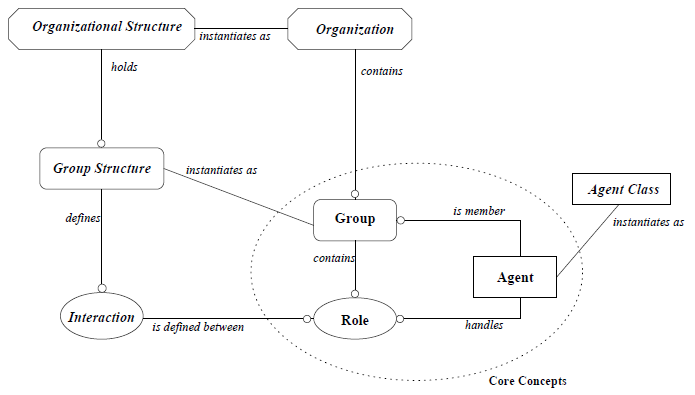
\includegraphics[width=0.75\textwidth]{images/aalaadin-metamodel.png}
	\caption{The Aalaadin metamodel}
	\label{figure:aalaadin-metamodel}
\end{figure}

\subsubsection*{Group Structure}

% Group structure - definition
A \textit{group structure} is an abstract description of a group \cite{Ferber97}.
It identifies all roles comprising the group and defines interactions among them.

% Group structure - definition characteristics
A group structure is defined by:
\begin{itemize}
	\item a list of available roles (see role definition) that can be played by agents in the group,
	\item a set of valid interaction schemes (including language) among roles.
\end{itemize}

% Group structure - partial instantiation
Note that a group might be a partial instantiation of its defining group structure.
This means that some roles defined in the group structure might not be played at the moment in the group.
This dynamic nature of groups allows for a great deal of run-time flexibility.
Contrast this with plain vanilla MAS where an agent, once an instance of a particular agent class, can not change this class at run-time.

\subsubsection*{Organizational Structure}

% Organizational structure - definition
The \textit{organizational structure}, as defined in \cite{Ferber97}, is a set of group structures expressing the design of a multiagent organization scheme.

% Organizational structure - about
The organizational structure can be seen as the specification of the problem to be solved (organization to be modelled) using a MAS.
Any sort of heterogeneity within a single system (e.g. agent architecture or language heterogeneity) can be managed by different group structures involved in the organizational structure.

% Organizational structure - partial instantiation
Similarly to groups, the actual organization is just one possible manifestation of the organizational structure.
Some groups defined in the organizational structure might not be present currently in the organization.
This also contributes to the overall run-time flexibility.

%%%%%%%%%%%%%%%%%%%%%%%%%%%%%%%%%%%%%%%%%%%%%%%%%%%%%%%%%%%%%%%%%%%%%%%%%%%%%%%%
\subsection{MadKit}

% MadKit - authors & references
The authors of Aalaadin/AGR also developed what started out as a proof-of-concept agent platform called \textbf{MadKit} (Multi-Agent Development Kit).
It has been described in an (unpublished) research report \cite{Ferber97} and a conference/workshop articles \cite{Ferber98} and \cite{Gutknecht00}.

%MadKit - design principles
The \textbf{MadKit} platform implements the Aalaadin/AGR core model and follows three design principles \cite{Ferber97}:
\begin{itemize}
	\item micro-kernel architecture,
	\item agentification of services and
	\item graphic component model.
\end{itemize}

% MadKit - basic philosophy
The basic philosophy of the Aalaadin/MadKit architecture is to use the platform itself for its own management wherever possible.
All services except for the most fundamental ones provided by the micro-kernel are implemented as agents, organized in groups and identified by roles \cite{Ferber98}.

% MadKit - technical details and requirements
\textbf{MadKit} is written in the Java programming language and runs on the Java platform, version 1.1.

%%%%%%%%%%%%%%%%%%%%%%%%%%%%%%%%%%%%%%%%%%%%%%%%%%%%%%%%%%%%%%%%%%%%%%%%%%%%%%%%
%% O&P                                                                        %%
%%%%%%%%%%%%%%%%%%%%%%%%%%%%%%%%%%%%%%%%%%%%%%%%%%%%%%%%%%%%%%%%%%%%%%%%%%%%%%%%
\section{O\&P}

% O&P - references
This section introduces the O&P\footnote{The metamodel was not given a name by its authors; we will, for the purposes of this thesis, call it ``O\&P''.} metamodel described in \cite{Odell01}, \cite{Parunak02}, \cite{Odell03b}, \cite{Odell04b} and \cite{Odell05}.
The overview presented here is due to \cite{Odell05} in particular.

% O%P - authors
O&P has been put forward in 2001 by James J. Odell, H. van Dyke Parunak and their colleagues.

%% Summary %%%%%%%%%%%%%%%%%%%%%%%%%%%%%%%%%%%%%%%%%%%%%%%%%%%%%%%%%%%%%%%%%%%%%

- PIM

%%%%%%%%%%%%%%%%%%%%%%%%%%%%%%%%%%%%%%%%%%%%%%%%%%%%%%%%%%%%%%%%%%%%%%%%%%%%%%%%
\subsection{Integrated Model}

% Integrated model - about
Figure~\ref{figure:onp-metamodel} shows the integrated model proposed in \cite{Odell05}.
The following subsections will focus on parts of the integrated model that can be studied in isolation.
We present the full model before discussing its parts (ALT: portions, sections) so that the reader can follow the discussion with assumption about where the part fits.

% Figure: O&P metmodel
\begin{figure}[ht]
	\centering
	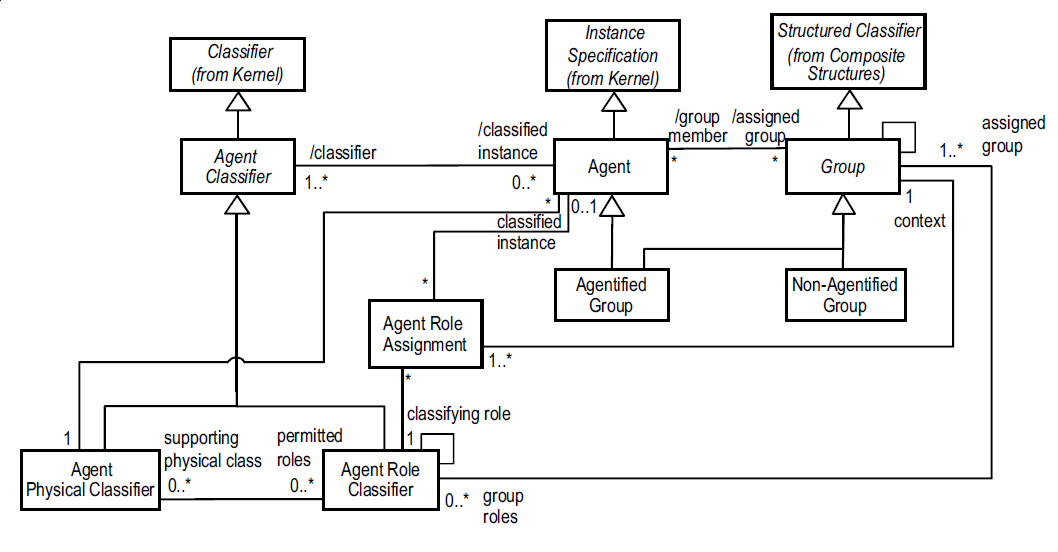
\includegraphics[width=0.75\textwidth]{images/onp-metamodel.png}
	\caption{The O\&P metamodel}
	\label{figure:onp-metamodel}
\end{figure}

% UML Classifier vs. UML Class
To understand the integrated model, it is essential to differentiate between the \textit{Classifier} and the \textit{Class} UML classes.
In short, Classifier does not have features that are associated with a OOP class (e.g. attributes, inheritance or interfaces).
On the other hand, the Class has these features.
Class is in fact a specialization of Classifier.
It is important to make this distinction, because the agent classification is based on an extension of Classifier, not Class.
The reason for this is that the authors did not want to impose object-orientation upon their metamodel.
After all, it is not at all expected of an agent to exhibit behaviour intrinsic to an object (e.g. polymorphism). 

%%%%%%%%%%%%%%%%%%%%%%%%%%%%%%%%%%%%%%%%%%%%%%%%%%%%%%%%%%%%%%%%%%%%%%%%%%%%%%%%
\subsection{Agent Classifiers and Agent}

\textit{Agent Classifier} is a UML Classifier that specifically provides a way to classify Agent instances by a set of features that they have in common \cite{Odell05}.
Classification is important because it enables a common definition of a set of entities that are in some sense similar, i.e. share some features and/or capabilities.

Figure~\ref{figure:onp-agent-classifiers} shows \textsc{Agent Classifier} and its two specializations: \textsc{Agent Physical Specifier} (alias \textsc{Physical Classifier}) and \textsc{Agent Role Specifier} (alias \textsc{Role Classifier}).

\begin{figure}[ht]
	\centering
	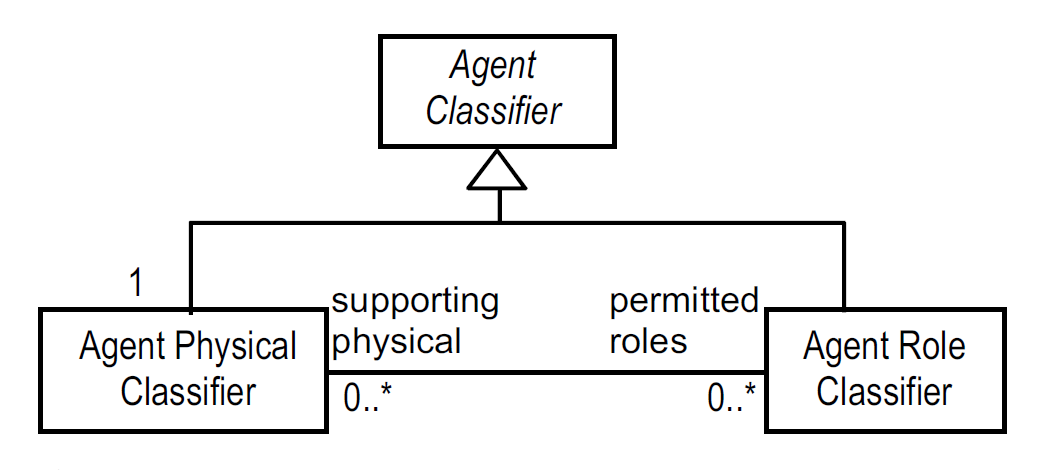
\includegraphics[width=0.5\textwidth]{images/onp-agent-classifiers.png}
	\caption{\textsc{Agent Classifier} and its two specializations: \textsc{Agent Physical Classifier} and \textsc{AGent Role Classifier}}
	\label{figure:onp-agent-classifiers}
\end{figure}

\subsubsection*{Agent Physical Classifier}

% Physical classifier - definition
The purpose of \textsc{Agent Physical Classifier} is to define a set of core features that an agent classified with it has independent of roles it plays \cite{Odell05}.
Every agent must be classified with exactly one physical classifier \footnote{Compare this with OOP, where an object must be an instance of exactly one class.} and is almost never reclassified during its lifetime.

% Physical classifiers vs. role classifiers
Figure~\ref{figure:onp-physical-classifier-examples} illustrates some examples of physical classifiers forming a (class?) hierarchy.
In comparison to role classifiers, physical classifiers attribute primary and permanent features to agents.
An example of a physical classifier from the real world would be `Human' agent.

% Figure: Physical classifer examples
\begin{figure}[ht]
	\centering
	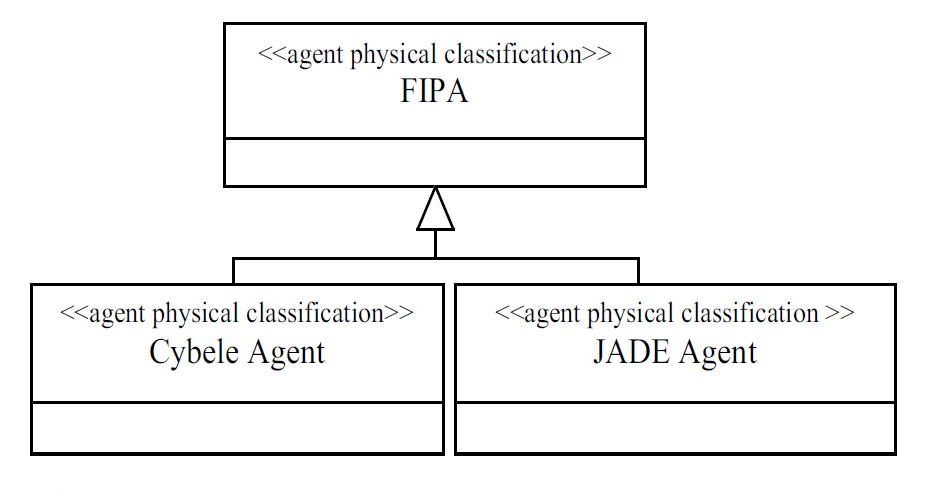
\includegraphics[width=0.5\textwidth]{images/onp-physical-classifier-examples.png}
	\caption{Examples of physical classifiers forming a (class?) hierarchy}
	\label{figure:onp-physical-classifier-examples}
\end{figure}

\subsubsection*{Agent Role Classifier}

% Role classifier - definition
The \textsc{Agent Role Classifier} is a classifier that defines a set of peripheral (as opposed to core) features that an agent classified with it has.
An agent can be classified with more than one role classifier at once (\textit{multiple classification}) and can be reclassified over time (\textit{dynamic classification}).

% Role hierarchy vs. class hierarchy
Figure~\ref{figure:onp-role-classifier-examples} depicts a small (class?) hierarchy of role classifiers.
In AUML, they are marked with the <<agent role>> stereotype.
In comparison to physical classifiers, role classifiers ascribe secondary and transient features to agents.
An example of a role classifier from the real world would be `Chess player' agent.

% Figure: Role classifer examples
\begin{figure}[ht]
	\centering
	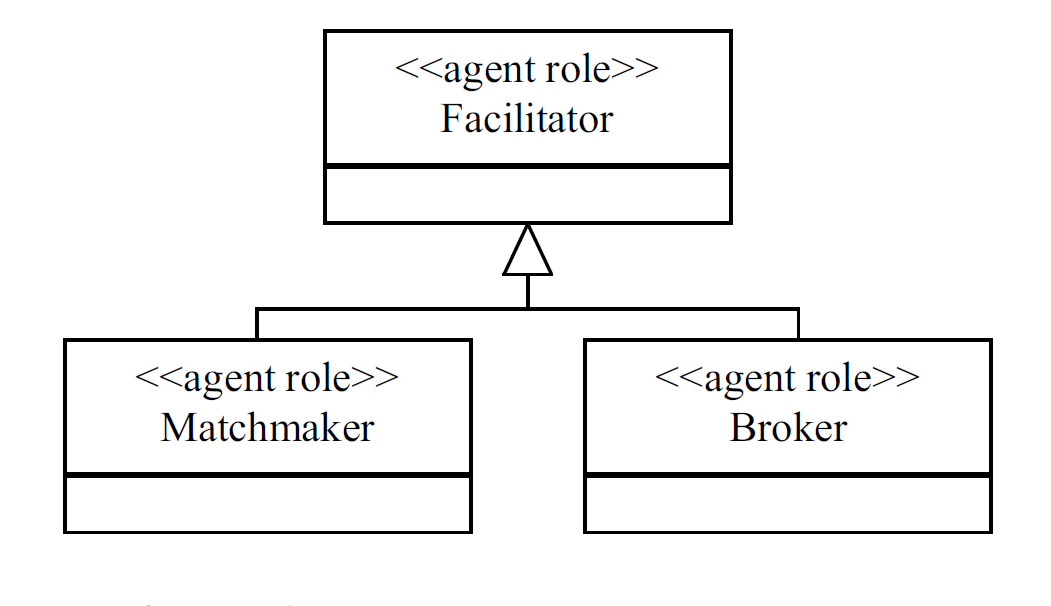
\includegraphics[width=0.5\textwidth]{images/onp-role-classifier-examples.png}
	\caption{Examples of role classifiers forming a (class?) hierarchy}
	\label{figure:onp-role-classifier-examples}
\end{figure}

\subsubsection*{Agent}

In O\&P, the basic concepts are \textsc{Agent Classifier} and \textsc{Agent}.
These modelling constructs are considered fundamental, because they enable a MAS designer to model \textit{agents classes} and \textit{agent instances} respectively.
Agent classes are the design-time (ALT: compile-time?) constructs providing the classification (features) of the actual run-time constructs - agent instances.
Said differently, an agent classifier defines features (state and behaviour) the the associated agents have. 

% TODO: Consider deleting this paragraph.
An \textsc{Agent} instance describes an agent.
This description can be incomplete; the purpose of an \textsc{Agent} instance is to only show what is of interest about an agent in the modelled MAS \cite{Odell05}.

% Figure - about
Figure~\ref{figure:onp-agent-examples} shows two \textsc{Agent} instances: \texttt{Agent4} and \texttt{Agent2}.
Agents may be linked via the roles they play.
In this scenario, \texttt{Agent4} is a broker and brokers something for \texttt{Agent2} who is a seller.

% Figure: Agent examples
\begin{figure}[ht]
	\centering
	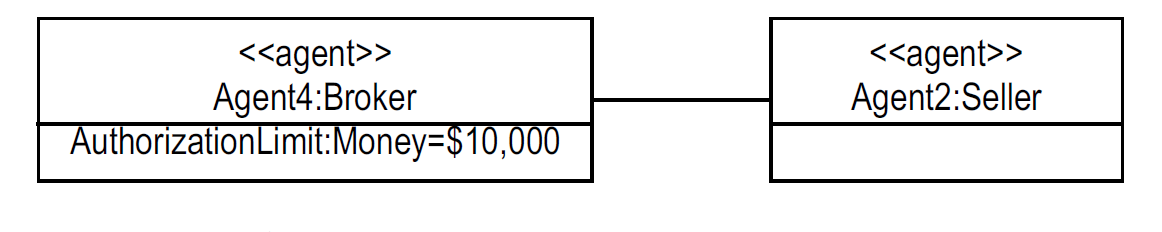
\includegraphics[width=0.5\textwidth]{images/onp-agent-examples.png}
	\caption{Examples of (linked) agents}
	\label{figure:onp-agent-examples}
\end{figure}

\subsubsection*{Association between Agent Physical Classifier and Agent Role Classifier}

The association between \textsc{Agent Physical Classifier} and \textsc{Agent Role Classifier} specifies which role classifiers are permitted for each physical classifier, independent of the capabilities of the individual agents classified with that that particular physical classifier \cite{Odell05}.

Figure~\ref{figure:onp-physical-classifier-role-classifier-association} illustrates the association between \textsc{Agent Physical Classifier} and \textsc{Agent Role Classifier}. It shows instances of \textsc{Agent Physical Classifier}: \texttt{JADE Agent Classifier} and \texttt{Cybele Agent Classifier}; and instances of \textsc{Agent Role Classifier}: \texttt{Manager}, \texttt{Broker}, \texttt{Trust Manager} and \texttt{Buyer}.
The \texttt{JADE Agent Classifier} physical classifier allows the \texttt{Manager} and \texttt{Broker} role classifiers to be played by JADE agents.
Similarly, the \texttt{Cybele Agent Classifier} physical classifier allows the \texttt{Broker}, \texttt{Trust Manager} and \texttt{Buyer} role classifiers to be taken on by Cybele agents.

% Figure: Agent physical classifier to Agent role classifier association
\begin{figure}[ht]
	\centering
	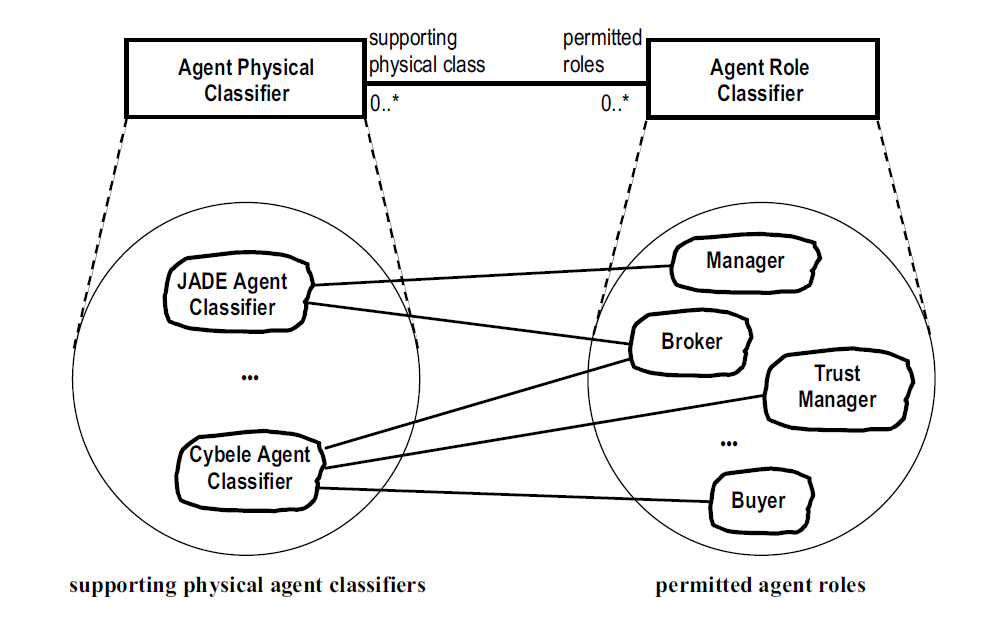
\includegraphics[width=0.75\textwidth]{images/onp-physical-classifier-role-classifier-association.png}
	\caption{The association between \textsc{Agent Physical Classifier} and \textsc{Agent Role Classifie}}
	\label{figure:onp-physical-classifier-role-classifier-association}
\end{figure}

\subsubsection*{Association between Agent and Agent Classifier}

The links of an agent with its agent classifiers (physical and role) determine its features.
Each agent classifier classifies an agent as a member of a set of agents sharing some physical or role-related features.

Figure~\ref{figure:onp-agent-agent-classifier-association} shows four instances of the \textsc{Agent} class: \texttt{Agent1}, \texttt{Agent2}, \texttt{Agent3} and \texttt{Agent4}; two instances of \textsc{Agent Physical Classifier}: \texttt{JADE Agent Classifier} and \texttt{Cybele Agent Classifier}; and four instances of \textsc{Agent Role Classifier}: \texttt{Manager}, \texttt{Buyer}, \textsc{Trust Manager} and \texttt{Broker}.
The links represent classification; for example \texttt{Agent1} is classified with \texttt{JADE Aget Classifier} agent physical classifier to be a JADE agent and with \texttt{Manager} agent role classifier to be a manager. 

% Figure: Agent to Agent Classifier association
\begin{figure}[ht]
	\centering
	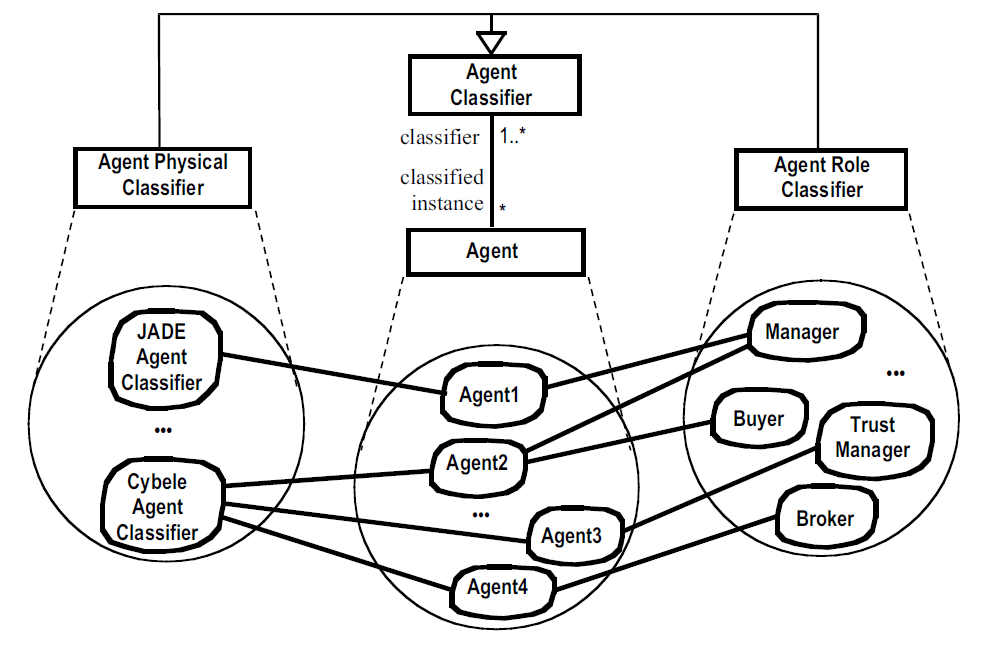
\includegraphics[width=0.75\textwidth]{images/onp-agent-agent-classifier-association.png}
	\caption{The association between \textsc{Agent} and \textsc{Agent Classifiers}}
	\label{figure:onp-agent-agent-classifier-association}
\end{figure}

% Physical vs. role classification
Observe the two main differences between the physical and role classification. First, the role classification is \textit{multiple} whereas the physical classification is \textit{single}.
While an agent can be classified with more than one (or even none) role classifiers at the same time, it must be classified with exactly one physical classifiers.
Second, the role classification is \textit{dynamic} in contrast to physical classification, which is \textit{static}.
Dynamic classification means that an agent can be declassified or reclassified with another role after initial classification. On the contrary, the physical classification is invariable in time
(``Once a JADE agent, always a JADE agent.'').

%%%%%%%%%%%%%%%%%%%%%%%%%%%%%%%%%%%%%%%%%%%%%%%%%%%%%%%%%%%%%%%%%%%%%%%%%%%%%%%%
\subsection{Group, Agentified Group and Non-agentified Group}

% Group - definition
A \textit{group} is a set of agents that are related via their roles, where these links must form
a connected graph within the group \cite{Odell05}.
This is the agent-centric way to look at at a group.
Another way of looking at a group is the role-centric way, which says that a group is a composite structure consisting of interrelated roles, where each of the group's roles has any number of agent instances \cite{Odell05}.

% Group - motivation
A group can be formed to exploit the synergies of its members, resulting in an entity capable of performing processes that none of its constituent agents (ALT: constituents) is capable.

\subsubsection*{Group Metamodel}

Figure~\ref{figure:onp-group} shows the \textsc{Group} class and its associations with \textsc{Agent} and \textsc{Role}.
The abstract \textsc{Group} class extends the UML Structured Classifier, which means that \textsc{Group} is defined as composite structure \footnote{In UML, Structured Classifier can be thought of as a structured set of classifiers. From this perspective, \textsc{Group} is a structured set of \textsc{Agent Role Classifiers}}.

% Figure: Group
\begin{figure}[ht]
	\centering
	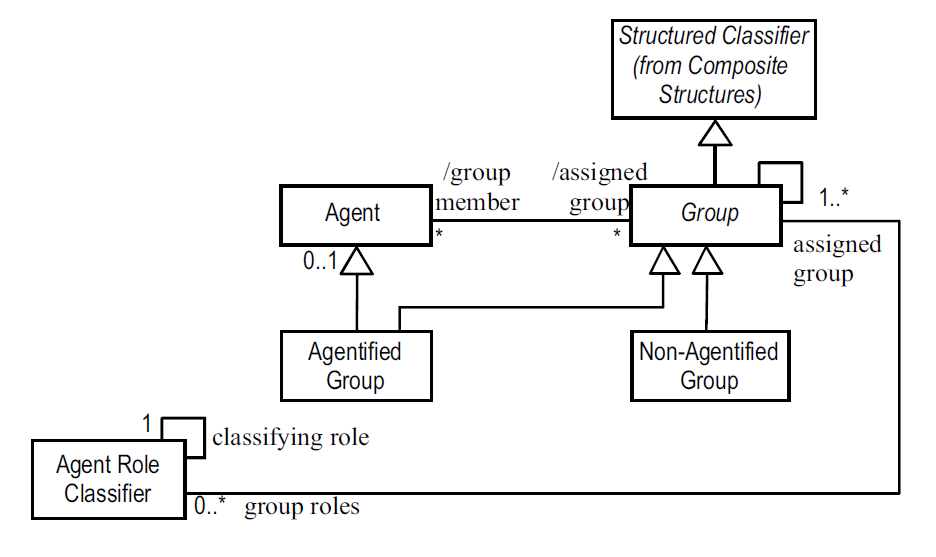
\includegraphics[width=0.75\textwidth]{images/onp-group.png}
	\caption{The \textsc{Group} class and its associations}
	\label{figure:onp-group}
\end{figure}

% Association between Group and Agent
Conceptually, a group consists of a set of agents playing roles within this group.
The roles that the agents can play (within this group) are represented by one or more agent role classifiers associated with this group.
Therefore, the set of agents comprising a group can be derived from the group via the agent role classifiers \cite{Odell05}.

\subsubsection*{Association between Group and Role}

% Association between Group and Agent Role Classifier
Figure~\ref{figure:onp-group-role-association} illustrates the association between groups and roles played in them by agents.
Observe that groups containing no roles is not allowed, each group must contain at least one role.
The opposite direction of the association requires each role to be contained in at least one group, since roles only make sense within context of a group.

% Figure: Group to Role association
\begin{figure}[ht]
	\centering
	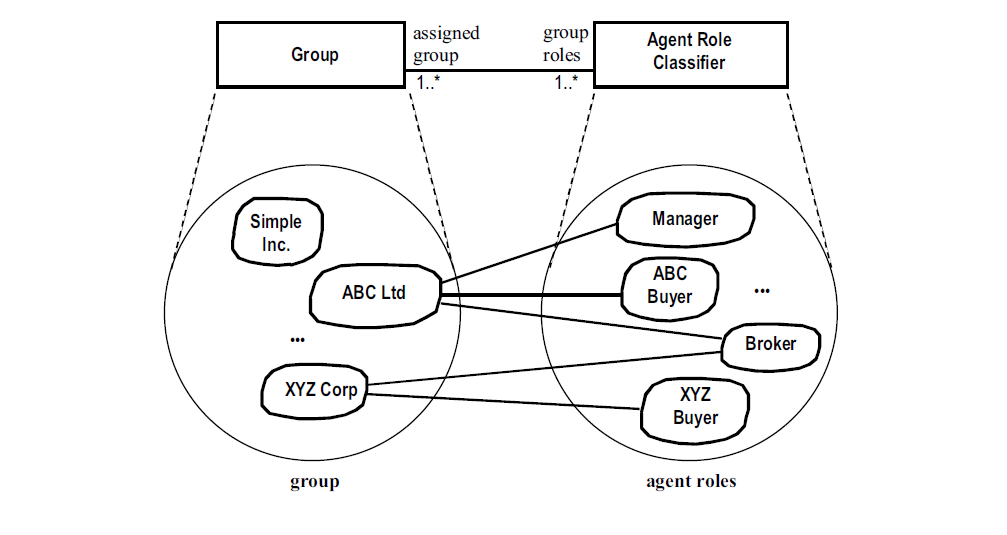
\includegraphics[width=0.75\textwidth]{images/onp-group-role-association.png}
	\caption{The association between \textsc{Group} and \textsc{Role}}
	\label{figure:onp-group-role-association}
\end{figure}

\subsubsection*{Agentified and Non-Agentified Groups}

The O\&P metamodel defines two types of groups: agentified and non-agentified.

% Agentified group
An \textit{agentified group} is a group that is also an agent in its own right, i.e. with its own interactive capability \cite{Odell05}.
This means that an agentified group can communicate with other agents (or agentified groups for that matter) directly, i.e. without a representative agent.
It can also be a member of other groups (agentified or not) and play roles, like any other agent.
To achieve this in the O\&P metamodel, \textsc{Agentified Group} is a subclass of both \textsc{Group} and \textsc{Agent} classes.
Figure~\ref{figure:onp-agentified-group} shows an example of an agentified group.
Notice the <<agent>> stereotype used to mark the group as agentified.

% Figure: agentified group
\begin{figure}[ht]
	\centering
	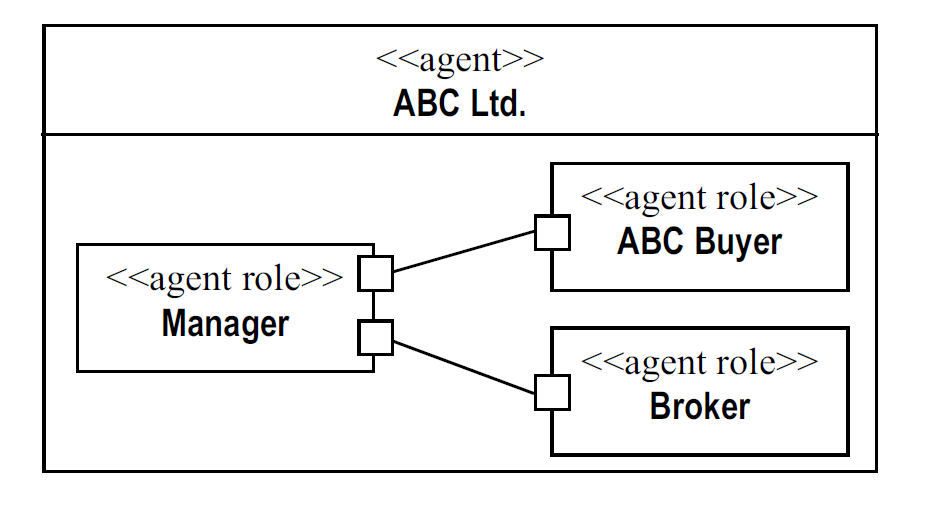
\includegraphics[width=0.5\textwidth]{images/onp-agentified-group.png}
	\caption{An example of an agentified group}
	\label{figure:onp-agentified-group}
\end{figure}

% Non-agentified group
A \textit{non-agentified group}, while still being a first-class citizen, is not an agent by itself, i.e. is it does not posses any capability to interact.
This kind of group always communicates with other agents (including agentified groups) through one of its members acting as an intermediary.
This is achieved in the O\&P metamodel by \textsc{Non-Agentified Group} extending only the \textsc{Group} class and not the \textsc{Agent} class.
An example of a non-agentified group is shown in figure~\ref{figure:onp-non-agentified-group}.
Note that this time there is no <<agent>> stereotype marking the group as agentified.

% Figure: non-agentified group
\begin{figure}[ht]
	\centering
	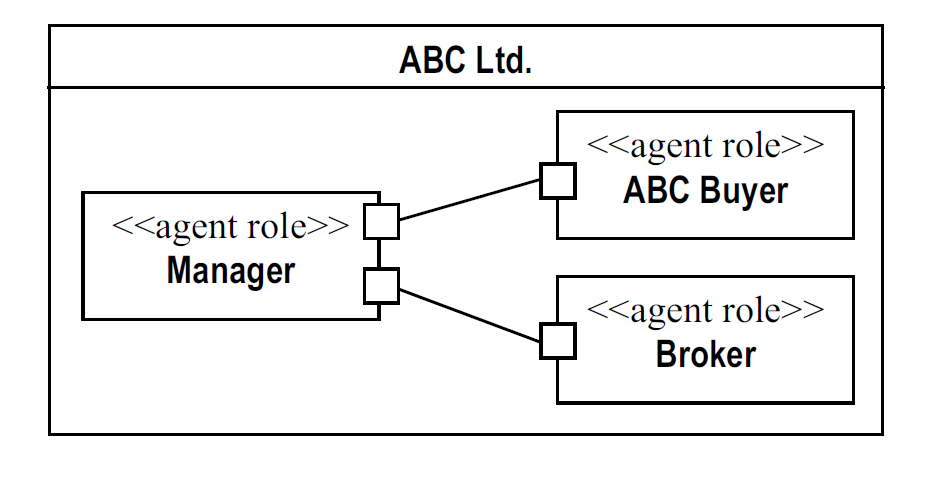
\includegraphics[width=0.5\textwidth]{images/onp-non-agentified-group.png}
	\caption{An example of a non-agentified group}
	\label{figure:onp-non-agentified-group}
\end{figure}

%%%%%%%%%%%%%%%%%%%%%%%%%%%%%%%%%%%%%%%%%%%%%%%%%%%%%%%%%%%%%%%%%%%%%%%%%%%%%%%%
\subsection{Agent Role Assignment}

The assignment of roles to agents is dynamic, i.e. it changes in time, and is modelled by \textit{Agent Role Assignment}.
Figure~\ref{figure:onp-agent-role-assignment} shows Agent Role Assignment and its associations.  

% Figure: Agent Role Assignment class
\begin{figure}[ht]
	\centering
	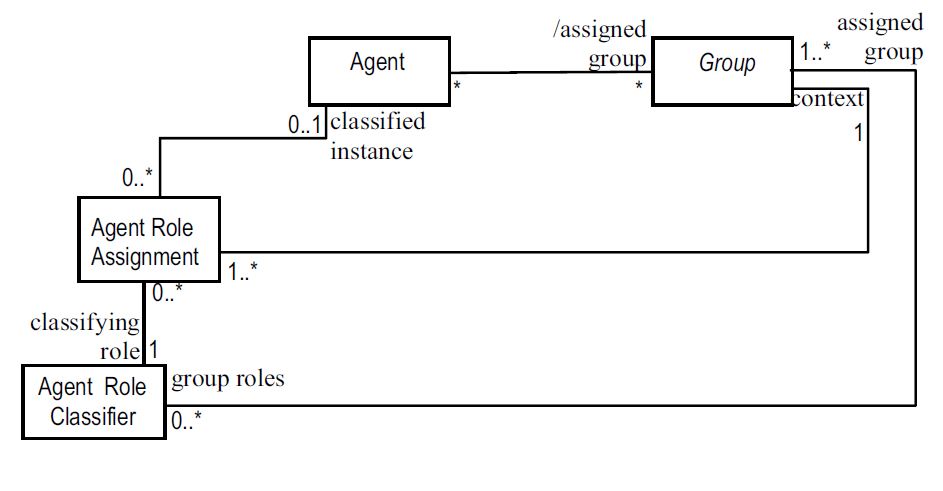
\includegraphics[width=0.75\textwidth]{images/onp-agent-role-assignment.png}
	\caption{The \textsc{Agent Role Assignment} class and its associations}
	\label{figure:onp-agent-role-assignment}
\end{figure}

\subsubsection*{Agent Role Assignment as a Ternary Association}

A direct association between Agent and Agent Role Classifier would represent that agents play roles.
However, such model would not be able to represent a situation where an agent plays a role in one group and does not play it in another.
To model this kind of situations, it is necessary to augment the agent-to-role association with a group context.
This yields a ternary association, promoted to (ALT: reified as) the Agent Role Assignment class.
Each instance of the Agent Role Assignment class associates an agent, role and a group.

\subsubsection*{Position}

It is possible to associate a group with a role leaving out an agent.
Such association is called a \textit{position} and models a situation where a concrete agent playing a role within a particular group is yet to be determined.
This turns out to be an extremely useful modelling concept, since more often than not, the organization modeller does not know (or simply does not care) which agent actually takes up a particular position when the MAS is run.
One more way to look at the \textsc{Agent Role Assignment} class is to view it as a reified association between the (potential) \textsc{Position} and \textsc{Agent} classes.

%%%%%%%%%%%%%%%%%%%%%%%%%%%%%%%%%%%%%%%%%%%%%%%%%%%%%%%%%%%%%%%%%%%%%%%%%%%%%%%%
%% PIM4Agents                                                                 %%
%%%%%%%%%%%%%%%%%%%%%%%%%%%%%%%%%%%%%%%%%%%%%%%%%%%%%%%%%%%%%%%%%%%%%%%%%%%%%%%%
\section{PIM4Agents}

% PIM4Agents - references
This section introduces the PIM4Agents\footnote{For `Platform-independent model for agents'.} metamodel described in \cite{Hahn07a}, \cite{Hahn07b} and \cite{Hahn08}.
We will present only a brief overview (particularly after \cite{Hahn07b}) since our work does not draw inspiration from PIM4Agents.

% PIM4Agents - authors
PIM4Agents has been proposed in 2007 by Christian Hahn, Cristián Madrigal-Mora and Klaus Fischer from German Research Centre for Artificial Intelligence (Deutsches Forschungszentrum f\"{u}r K\"{u}nstliche Intelligenz, DFKI).

%% Summary %%%%%%%%%%%%%%%%%%%%%%%%%%%%%%%%%%%%%%%%%%%%%%%%%%%%%%%%%%%%%%%%%%%%%

- PIM

% PIM4Agents & MDA
PIM4Agents has been specifically designed to be employed in the Model-driven engineering (MDE) software development methodology, more precisely the Model-driven architecture (MDA) by Object Management Group (OMG).
Apart from the platform-independent metamodel itself, the authors have proposed two platform-specific metamodels: JackMM (for JACK) and JadeMM (for JADE).
They have also described two sets of model transformations to convert platform-independent models (PIM) to platform-specific models (PSM): PIM4Agents to JackMM and PIM4Agents to JadeMM.

%%%%%%%%%%%%%%%%%%%%%%%%%%%%%%%%%%%%%%%%%%%%%%%%%%%%%%%%%%%%%%%%%%%%%%%%%%%%%%%%
\subsection*{Core Metamodel}

% Core metamodel
In order to support an evolution, the PIM4Agents metamodel is structured around a small core that could possibly be augmented with extensions to model specific (even unforeseen) aspects of MAS, for example security.
The core metamodel is shown in figure~\ref{figure:pim4agents-metamodel}.
The metamodel, like previous metamodels, is built around the concept of \textsc{Agent}, an autonomous entity capable of sensing and acting upon its environment.
Each \textsc{Agent} has access to a set of \textsc{Resources} from its surrounding \textsc{Environment}.

\textsc{Behaviour} can be primitive (ALT: simple) or composed of sub-behaviours; a whole hierarchy of specific \textsc{Behaviours} can be created.
\textsc{Behaviour} may also send or receive a \textsc{Message} according to a given \textsc{Protocol}.
\textsc{Capability} allows to group \textsc{Behaviours} that, conceptually, have a correspondence with regard to what they allow \textsc{Agent} to do.

\textsc{Role} is an abstraction of the social behaviour of the Agent in a given social context, usually \textsc{Cooperation}.
This \textsc{Role} specifies the responsibilities of \textsc{Agent} in that social context.
Correspondingly, \textsc{Cooperation} represents the interaction between \textsc{Agents} performing the required set of \textsc{Roles}.
The detailed realisation of this interaction is described by \textsc{Protocol} that indicates what are \textsc{Messages} to be expected from each of \textsc{Roles} at which point in time.
The execution of \textsc{Protocol} is performed by a set of \textsc{Behaviours}, each of which sends and/or receives \textsc{Messages} in accordance to its \textsc{Role}.

\textsc{Agents} can take part in \textsc{Organisation}, a special kind of \textsc{Cooperation} that also has the same characteristics as \textsc{Agent}.
Therefore, \textsc{Organisation} can perform roles and has \textsc{Capabilities} which can be performed by its members, be it \textsc{Agents} or sub-organisations.
The multiple inheritance of \textsc{Organisation} from \textsc{Agent} and \textsc{Cooperation} also allows it to have its own internal protocol that specifies how \textsc{Organisation} coordinates its members.

% Figure: PIM4Agents metamodel
\begin{figure}[ht]
	\centering
	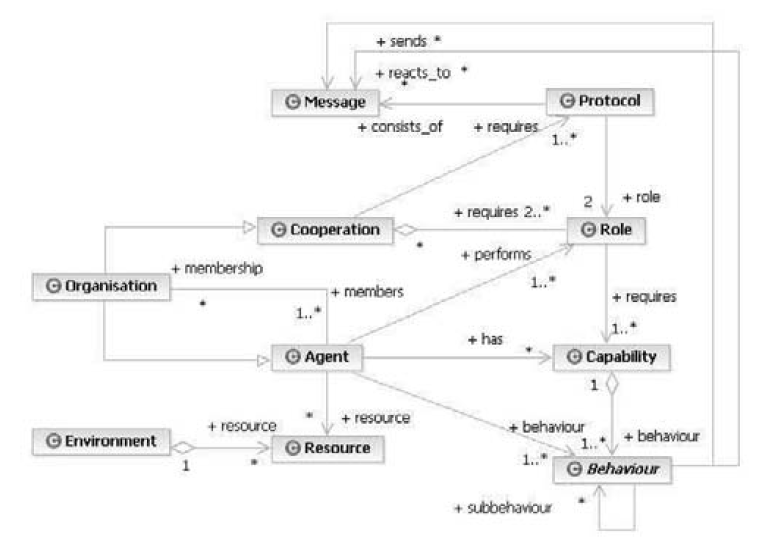
\includegraphics[width=\textwidth]{images/pim4agents-metamodel.png}
	\caption{The PIM4Agents metamodel}
	\label{figure:pim4agents-metamodel}
\end{figure}

%%%%%%%%%%%%%%%%%%%%%%%%%%%%%%%%%%%%%%%%%%%%%%%%%%%%%%%%%%%%%%%%%%%%%%%%%%%%%%%%
\subsection{JadeOrgs}

JadeOrgs is an extension of the JADE (agent?) platform that implements the JadeMM platform-specific metamodel.
JadeMM is defined using Eclipse Modeling Framework (EMF) to exploit EMF's code generation facility; given a platform-independent model of a MAS (conforming to PIM4Agents), the corresponding JADE/JadeOrgs platform-specific model (conforming to JadeMM) can be derived automatically.

JadeOrgs has been described in \cite{Madrigal-Mora08} and \cite{Madrigal-Mora09}.

%%%%%%%%%%%%%%%%%%%%%%%%%%%%%%%%%%%%%%%%%%%%%%%%%%%%%%%%%%%%%%%%%%%%%%%%%%%%%%%%
%% powerJade                                                                  %%
%%%%%%%%%%%%%%%%%%%%%%%%%%%%%%%%%%%%%%%%%%%%%%%%%%%%%%%%%%%%%%%%%%%%%%%%%%%%%%%%
\section{powerJade}

% powerJade - references
This section introduces the powerJade\footnote{Intentionally uncapitalized.} metamodel described in \cite{Baldoni08a}, \cite{Baldoni08b}, \cite{Baldoni09} and \cite{Baldoni10}.
The presented overview is due to \cite{Hahn07b} in particular.

% powerJade - authors
powerJade has been put forward in 2008 by Matteo Baldoni, Guido Boella and their colleagues from University of Turin in Turin, Italy.

%% Summary %%%%%%%%%%%%%%%%%%%%%%%%%%%%%%%%%%%%%%%%%%%%%%%%%%%%%%%%%%%%%%%%%%%%%

% powerJade inspired by powerJava
powerJade is a platform independent metamodel inspired by the authors' previous work on powerJava - the extension of the Java programming language with an explicit role construct based on an ontological analysis of roles (see \cite{Baldoni05}, \cite{Baldoni06a}, \cite{Baldoni06b} and \cite{Baldoni07}).

% Definitions (organization, role)
An organization (or, more generally, an institution) belongs to the social reality and it can only be interacted with via the roles it contains \cite{Boella06}.
It is not an object (as in OOP) that could be manipulated from outside.
The (modelling?) concept of an \textit{organization} is not only advantageous when modelling problem domains including organizations/institutions of some kind.
Indeed, we can view every object (as in OOP) as an organization/institution offering different ways of interacting with it, each of which is represented by a different role.

%%%%%%%%%%%%%%%%%%%%%%%%%%%%%%%%%%%%%%%%%%%%%%%%%%%%%%%%%%%%%%%%%%%%%%%%%%%%%%%%
\subsection*{Organization Structure Metamodel}
% ALT: Ontological Model of an Organization, Organization Ontology

An ontological analysis of roles in \cite{Boella04} yields the following properties of roles:
\begin{itemize}
	\item \textit{Foundation} - a role instance is always associated with an instance of the organization class to which is belongs and with a player instance.
	\item \textit{Definitional dependence} - the role definition depends on the organizations it belongs to.
	\item \textit{Institutional powers} - the role operations (called \textit{powers}) have access to the state of the organization and other roles of the organization.
	\item \textit{Prerequisities} - to be granted (and play) a role, the player must be able to perform operations (called \textit{requirements}) which can be requested while it plays the role.
\end{itemize}

% Ontological status of organizations and roles compared to agents
The metamodel in \cite{Boella04} focuses on the organization structure.
The ontological status of organizations and roles \cite{Boella04} does not differ completely from that of agents (AOP) or objects (OOP).
On one hand, roles do not exist as independent entities (like objects in OOP), since they are necessarily linked to organizations.
Additionally, organizations and roles are not autonomous and act via players.
On the other hand, organizations and roles, like agents, are descriptions of complex behaviour.
In the real world, organizations are considered legal entities; they can even act like agents, although via a representative role.
Since they share some properties with agents, they can be modelled using similar primitives.

%%%%%%%%%%%%%%%%%%%%%%%%%%%%%%%%%%%%%%%%%%%%%%%%%%%%%%%%%%%%%%%%%%%%%%%%%%%%%%%%
\subsection*{Role Dynamics Metamodel}
% ALT: Ontological Model of Role Dynamics, Role Dynamics Ontology

The metamodel in \cite{Dastani04} is focused on role dynamics.
Four operations pertaining to the role dynamics are defined: \textit{enact} and \textit{deact} which mean that agent assumes (ALT: acquires) and relinquishes a role respectively, and \textit{activate} and \textit{deactivate} which mean the agent actually starts and stops playing (invoking powers) a role respectively.
Even though it is possible (and very common indeed) for an agent to be enacting multiple roles simultaneously, only one of these can be active at any moment.
Naturally, it is possible that none is active.
In particular, when an agent is invoking (ALT: performing, executing) a power, at that moment exactly one of its roles is active.

%%%%%%%%%%%%%%%%%%%%%%%%%%%%%%%%%%%%%%%%%%%%%%%%%%%%%%%%%%%%%%%%%%%%%%%%%%%%%%%%
\subsection*{Unified Model}

The authors of powerJade merged the metamodels in \cite{Boella04} (organization strucure) and \cite{Boella04} (role dynamics) to model \textit{open systems}\footnote{Open multiagent system is a system that agents can enter and/or leave.}.
Organizations and roles are not just design-time constructions (ALT: abstractions) and players are not isolated agents - the are all agents interaction with one another.
A logical specification of this unified model can be found in \cite{Boella07}.

%%%%%%%%%%%%%%%%%%%%%%%%%%%%%%%%%%%%%%%%%%%%%%%%%%%%%%%%%%%%%%%%%%%%%%%%%%%%%%%%
\subsection*{Powers and Requirements}

% Role (AOPwO) vs. interace (OOP)
Roles can be compared to interfaces from OOP; just like an interface is a contract between a calling class and called class, a role is a contract between an organization and an agent.

% Relationship between interface and implementing entity (class, player agent instance)
In OOP, the relationship between an interface and a class is a static one - the class definition (design-time) specifies a set of interfaces the class implements and no interfaces can be added or removed at run-time.
In contrast, the relationship between a role and a player agent instance in AOP with Organizations (AOPwO) is dynamic - the player agent instance definition (design-time) usually does not specify roles it plays, but it can enact and deact roles at run-time.

% Interface methods & events vs. role requirements & powers
Interfaces in OOP declare methods the implementing class must implement and events it may raise (ALT: fire, trigger).
Interface methods are the class' \textit{responsibilities} (what it \textit{must} do?) and the interface events are the class' \textit{competences} (what it \textit{can} do?).
Similarly, role \textit{requirements} are the responsibilities the player agent takes by enacting/activating the role and the role \textit{powers} are the competences they player gains by enacting/activating the role.
Thus, interface methods correspond to role requirements, while interface events are analogous to role powers.